\documentclass{scrreprt}

\usepackage[english,czech]{babel}
\usepackage[utf8]{inputenc}
\usepackage{graphicx}

\begin{document}

\setcounter{chapter}{7}
\chapter{Architektury softwarových systémů, komponentové architektury, vzdálená invokace, distribuované komponentové architektury (CORBA), redundance a návrh spolehlivých systémů. (A4B77ASS)}

\section{Nefunkční požadavky softwarových systémů}
Specifikace \textbf{ISO/IEC 9126}:
\begin{itemize}
\item \textbf{Functionality} – existence of a set of functions and their specified properties
\item \textbf{Reliability} - capability of software to \emph{maintain} its level of performance under stated conditions for a stated period of time
\item \textbf{Usability} - effort needed for use
\item \textbf{Efficiency} - relationship between the \emph{level of performance} of the software and the amount of \emph{resources} used, under stated conditions
\item \textbf{Maintainability} - effort needed to \emph{make specified modifications}
\item \textbf{Portability} - transferred from one \emph{environment} to another
\end{itemize}

\begin{center}
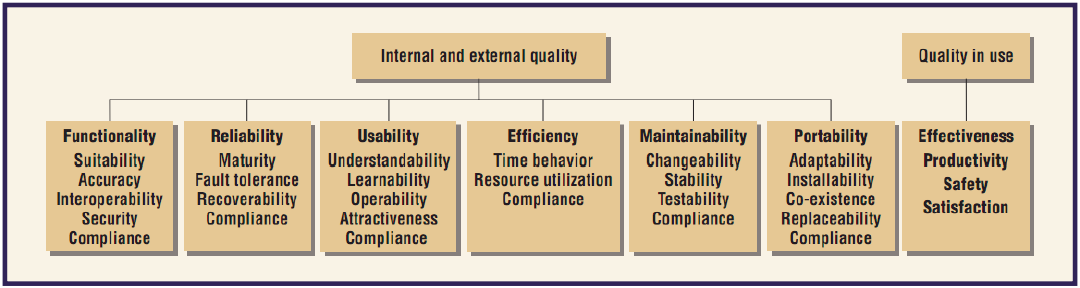
\includegraphics[width=\linewidth]{img/iso}
\end{center}

\section{Návrhové vzory pro distribuované systémy}
\begin{itemize}
\item \textbf{Façade} - zakrývá komplexitu a heterogenitu systému či knihovny za jednoduché rozhraní, často zakrývá více objektů
\item \textbf{Adapter/Wrapper} - poskytuje mapování mezi dvěma rozhraními se stejnou funkcionalitou, zaručuje kompatibilitu volání
\item \textbf{Wrapper Façade} - zapouzdřuje funkce a data poskytované ne-objektově orientovaným API pod objektově orientované rozhraní
\item \textbf{Proxy} - je lokální reprezentace vzdálených objektů, rozhraní nebo knihoven
\item \textbf{Active Object} - odděluje spouštění metody od její invokace, tím zlepšuje souběžnost a zjednodušuje synchronní přístup k objektům
\item \textbf{Reactor} - umožňuje událostmi řízeným aplikacím zpracovávání požadavků od jednoho či více klientů
\item \textbf{Proactor} - umožňuje událostmi řízeným aplikacím zpracovávání požadavků, které jsou vyvolány dokončením asynchronních operací
\item \textbf{HalfSync/HalfAsync} - odděluje synchronní a asynchronní zpracovávání v souběžných systémech
\end{itemize}

\section{Vzdálená invokace - RMI}
RMI (Remote Method Invocation) je způsob používání vzdálených objektů jako lokálních, dostupné jen pro Javu. Architektura klient-server: server vytvoří vzdálené objekty, klient tyto objekty získá a může na nich volat metody. Umožňuje načítat definice tříd za běhu.

Vzdálené objekty je možné předat jiné (klientské) VM pomocí reference, poté je na nich možné volat metody. Výpočet pak probíhá na VM serveru. Vzdálené objekty musí extendovat rozhraní \textsf{Remote} a všechny metody musí vyhazovat \textsf{RemoteException}. Rozhraní \textsf{Task} společné pro klienta i server definuje jejich vzájemnou komunikaci. Takto může server vykonávat jakékoliv úkoly, které implementují rozhraní \textsf{Task}, RMI pak za běhu načte definice tříd. Data přesouvané mezi klientem a servem musí být buď primitivní datové typy nebo objekty implementující \textsf{Serializable} nebo \textsf{Remote}.
\begin{verbatim}
public interface Task<T> {
    T execute();
}

public interface Compute extends Remote {
    <T> T perform(Task<T> t) throws RemoteException;
}
\end{verbatim}

\section{Distribuované komponenty - CORBA}
CORBA (Common Object Request Broker Architecture) je platformně a jazykově nezávislý standard (architektura) pro distribuované výpočty. Umožňuje transparentní invokaci objektů a metod přes síť.

\textbf{ORB} (Object Request Broker) přenáší žádosti od klienta na server a volá metody na vzdálených objektech, potom co server žádost zpracuje, tak ORB přenese odpověď zpět ke klientovi. Klient pak volá metody na lokální proxy. Pro komunikaci mezi jednotlivými ORB a pro přenos dat se používá \textbf{IIOP} (Internet Inter-ORB Protocol).

\textbf{IDL} (Interface Definition Language) je platformně a jazykově nezávislý objektově orientovaný jazyk určený ke specifikaci business level služeb a objektů. Používá se pro popis dostupných lokálních a serverových metod.

\begin{center}
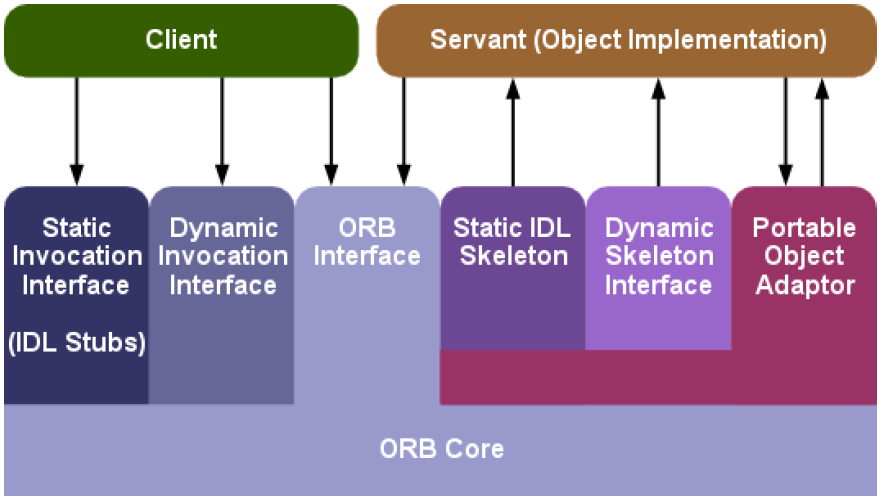
\includegraphics[scale=0.5]{img/corba}
\end{center}
\begin{center}
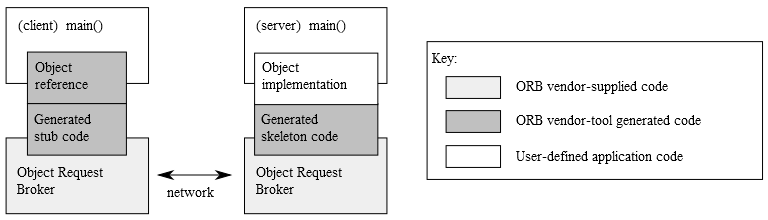
\includegraphics[scale=0.9]{img/orb}
\end{center}

\section{Masivně distribuované architektury}

\subsection{Map-Reduce}
Navržen a používán Googlem, masivně paralelní přístup založený a inspirovaný na funkcionálním programování. Používá se k ukládání, manipulaci a hledání v datech s jednoduchou strukturou, kterých je ale velké množství. Operuje nad dvojicemi klíč-hodnota. Metoda Map-Reduce má dvě opakující se fáze:
\begin{itemize}
\item[\textbf{1)}] \textbf{Map} - funkce (filtr) se aplikuje na množinu záznamů/elementů v listu
\item[\textbf{2)}] \textbf{Reduce} - zkrácení listu za použití nějaké agregační funkce
\end{itemize}
Z výpočetních jednotek je vybrán jeden řídící \emph{master node} a ostatní jsou \emph{worker nodes}. Masivní paralelizace je dosažena tím, že se data rozdělí do několika částí a nechají se zpracovat různým \emph{worker nodes}. Příklady použití: distribuované zpracování regulárních výrazu, počítání URL referencí, vytváření reverzního grafu webu, sémantické vyhledávání, invertovaní indexování, distribuované řazení.

\begin{center}
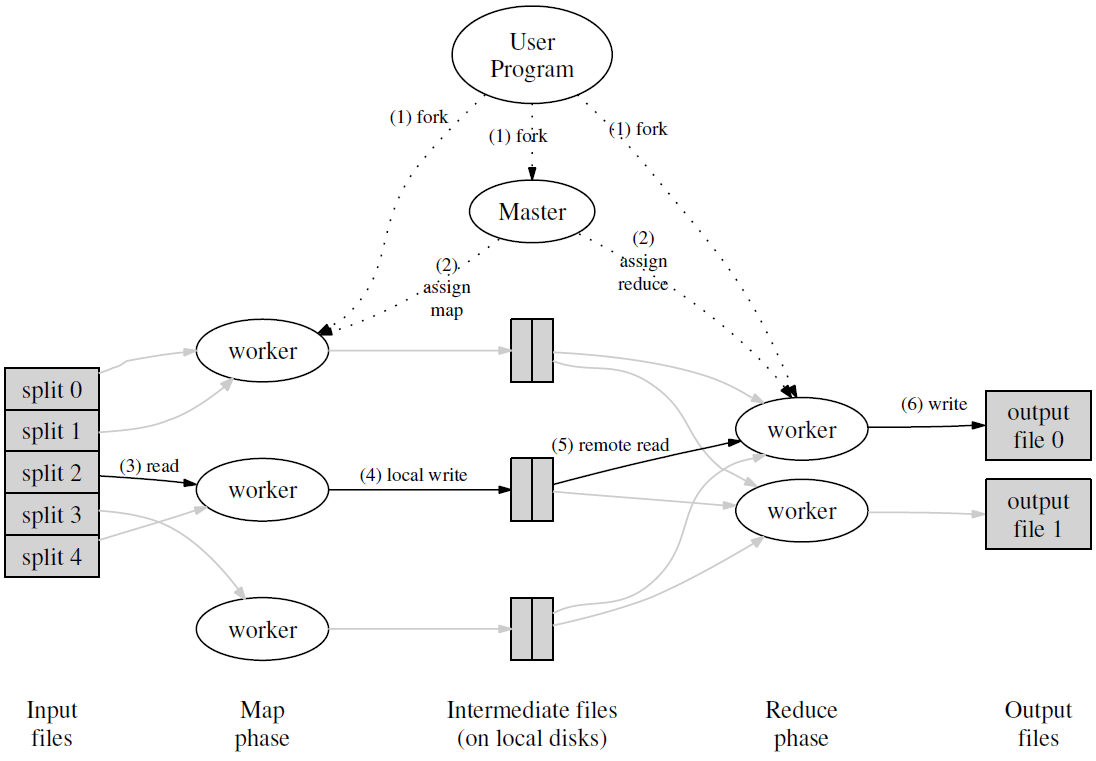
\includegraphics[width=\linewidth]{img/map_reduce}
\end{center}

\subsection{KaZaA}
Je skupina protokolů a technologií používaných pro \emph{peer-to-peer} komunikaci.
\begin{itemize}
\item \textbf{Napster} - \emph{peer-to-peer} síť s centralizovaným řídícím prvkem
\item \textbf{Gnutella} - Je \emph{flat peer-to-peer} síť kde jsou si všichni peery rovni. Při startu se vytvoří daný počet náhodných spojení s peery, které jsou v tu dobu aktivní. Peery sdílí informace o ostatních peerech. V novějších verzích představen koncept \emph{ultrapeerů} (peery s větším množstvím spojení, huby) - design ovlivněný \emph{scale-free} sítěmi.
\end{itemize}

\paragraph*{Scale-Free Networks} Sítě reflektující povahu reálného světa. Existují dva typy nodů - \emph{Ordinary Nodes} a \emph{Super Nodes}. Při startu se ON připojí k některému z dostupných SN. Každý SN si udržuje databázi připojených ON a aktuální topologii dalších SN. Při hledání se ON spojí s SN, ale jsou možné spojení přímo ON k ON (Skype).

\begin{center}
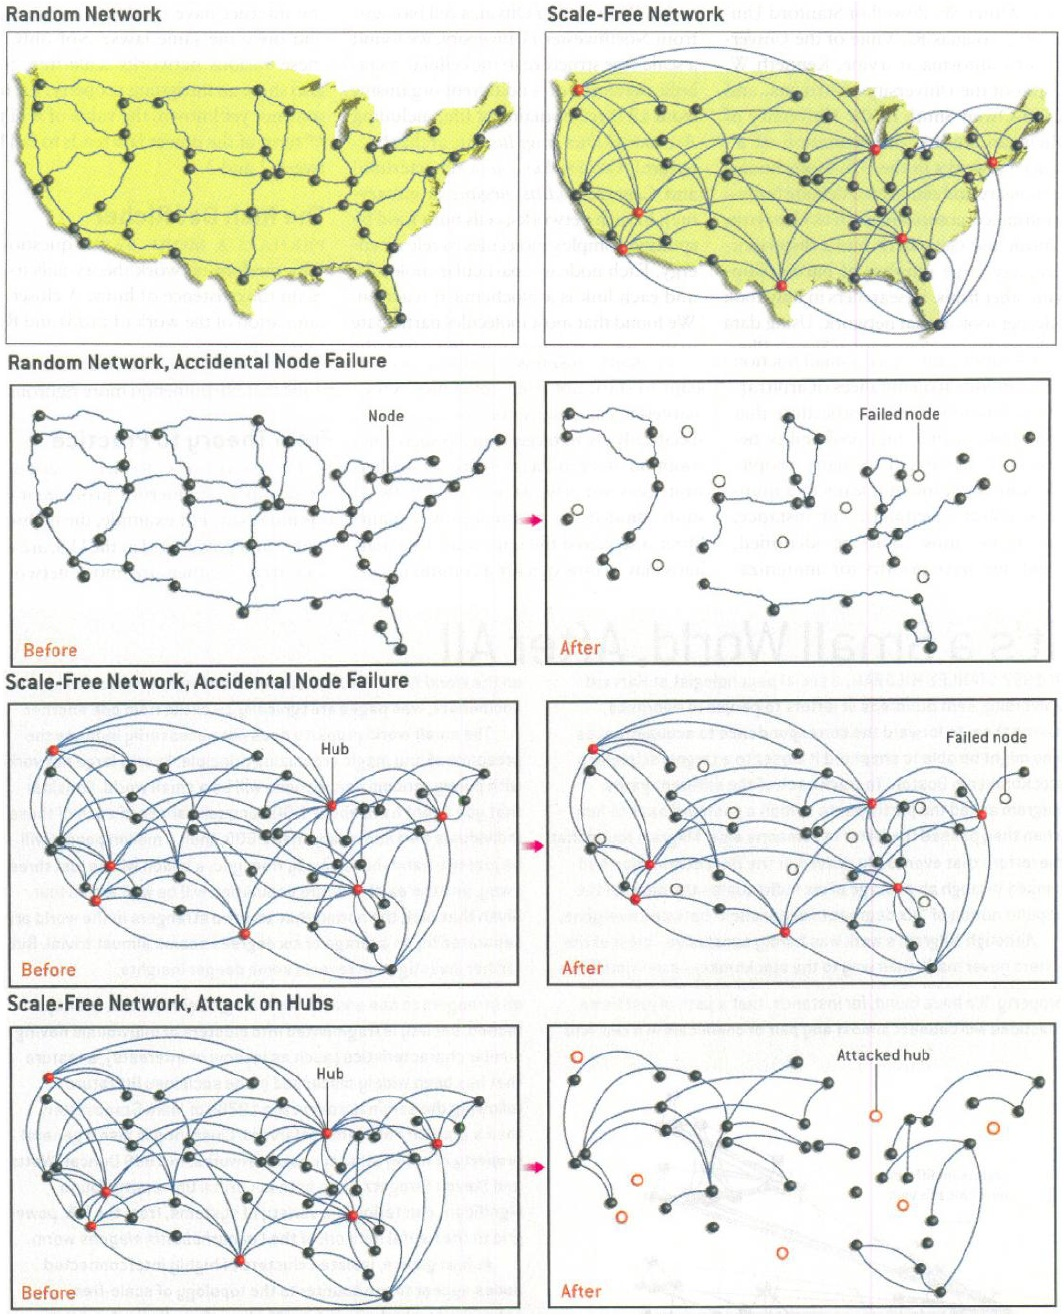
\includegraphics[width=\linewidth]{img/networks}
\end{center}

\end{document}
